\documentclass{article}

\usepackage{color}
\usepackage{graphicx}
\usepackage{amsmath}
\usepackage{indentfirst}
\usepackage{float}
\usepackage{siunitx}
\begin{document}
\vspace*{0.25cm}
\hrulefill
\thispagestyle{empty}

\begin{center}
\begin{large}
\sc{UM--SJTU Joint Institute \vspace{0.3em} \\ Ve215}
\end{large}

\hrulefill

\vspace*{5cm}
\begin{Large}
\sc{{Laboratory Report}}
\end{Large}

\vspace{2em}

\begin{large}
\sc{{Exercise 4
\vspace{0.5em}

AC Lab}}
\end{large}
\end{center}


\vfill

\begin{table}[h!]
\flushleft
\begin{tabular}{ll}
Name: Jin Minhao \hspace*{2em}&
ID: 516370910116\hspace*{2em}\\





Date: \today

\end{tabular}
\end{table}


\newpage
\section{Introduction}
\subsection{Objectives}
\begin{enumerate}
\item Learn how to define, calculate, and measure the amplitude of a sinusoidal
signal
\item Learn how to define, calculate, and measure the Rise Time and Fall Time of a
signal
\item Learn how to observe FFT spectra of signal and measure their parameters with
cursors
\item Measure the waveforms and FFT spectra of various signals
\item Compare your theoretical results obtained in the Pre-Lab with your In-Lab
data
\end{enumerate}
\subsection{Introduction}
\subsubsection{High-Z mode}
Here I want to introduce you what is the High-Z mode we have kept emphasizing
during the previous Labs.

You have already learnt Thevenin equivalent of a circuit. You can think the
function generator in terms of its Thevenin equivalent circuit, which includes the
voltage source and $V_S$ and the equivalent resistance of $50\Omega$ as shown below.
\begin{figure}[H]
	\centering
	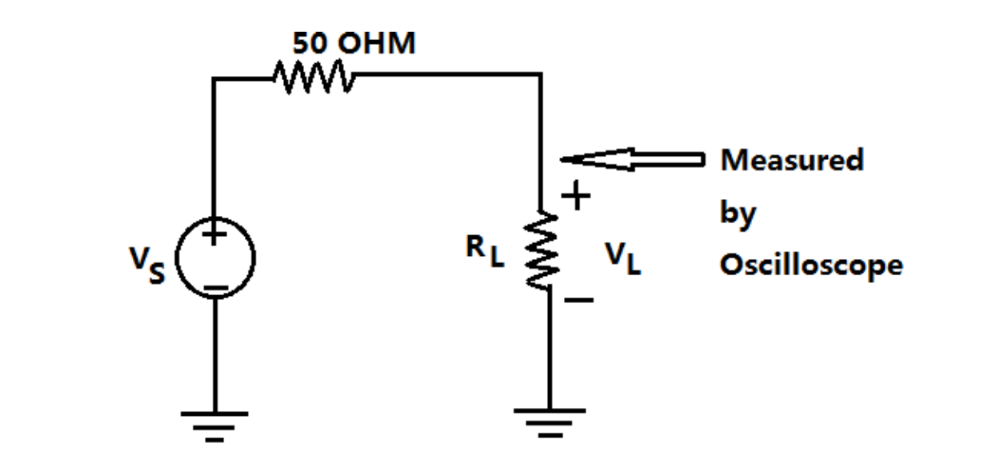
\includegraphics[width=0.7\linewidth]{p1}
	\label{fig:p1}
\end{figure}
When the load $R_L$ is $50\Omega$ , according to voltage division, we know that the $V_L$
measured will be $0.5V_S$. In this case, we use the 50 OHM mode, in which the
function generator produces voltage $V_S$ but displays voltage $0.5V_S$. In that way, if
you set $2V_{ppk}$ for the function generator, the actual $V_S$ will be $4V_{ppk}$ to make sure
the load get a voltage of $2V_{ppk}$. In our lab measurements, the load resistance $R_L$ is very high—the input resistance
of the oscilloscope is about $1 M\Omega$ . The $V_L$ measured across $R_L$ practically equals
$V_S$. So we use High Z mode, in which the function generator produce voltage $V_S$
and display
\subsubsection{The Rise Time and Fall Time of signals}
The Rise time is the interval between the moment of the time when the signal
reaches its $10\%$ level and the moment of time when the signal reaches its $90\%$.
We have already used this concept in our Lab3.
\begin{figure}[H]
	\centering
	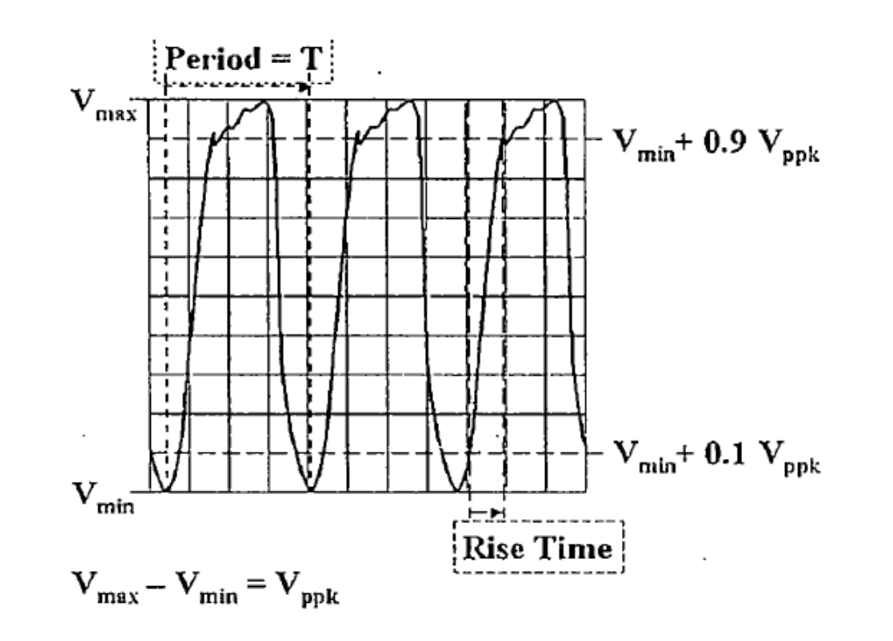
\includegraphics[width=0.7\linewidth]{p2}
	\label{fig:p2}
\end{figure}
\begin{figure}[H]
	\centering
	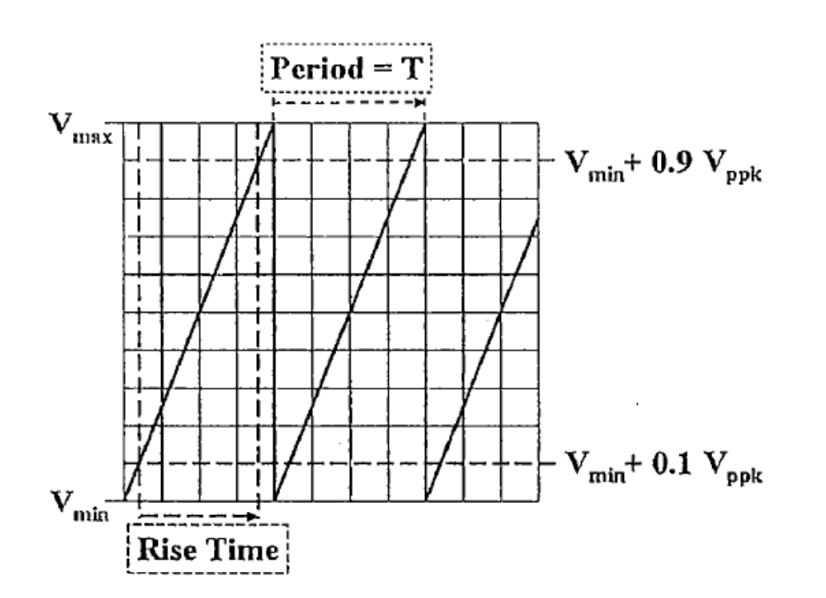
\includegraphics[width=0.7\linewidth]{p3}
	\label{fig:p3}
\end{figure}
The above two figures illustrate the rise time of a sinusoidal like wave and a
saw-tooth wave. If you do not know what is $V_{ppk}$, you can refer to part 4 of this
section.
Take the sinusoid wave as an example to calculate the rise time.
\begin{figure}[H]
	\centering
	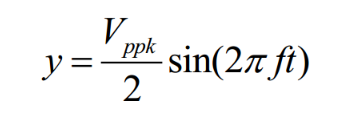
\includegraphics[width=0.2\linewidth]{p4}
	\label{fig:p4}
\end{figure}
\begin{figure}[H]
	\centering
	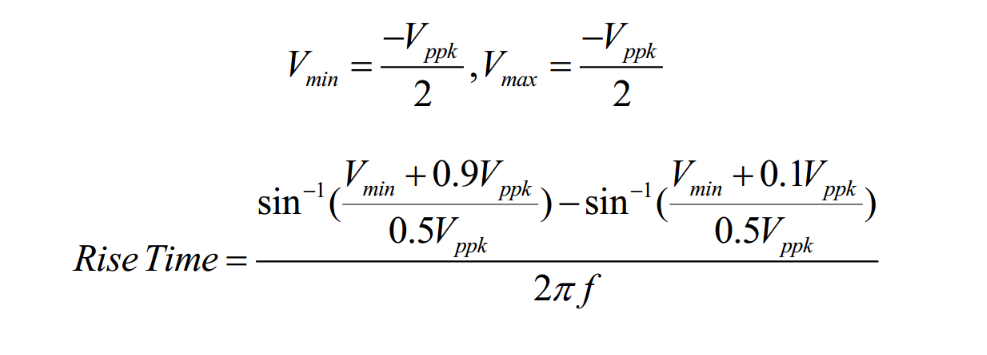
\includegraphics[width=0.4\linewidth]{p5}
	\label{fig:p5}
\end{figure}
\subsubsection{Fourier Series Representation of a Signal}
Here I am going to give you a general idea of Fourier Series to help you
understand some parts of this lab. You will learn Fourier Series in details in your
math course this semester.

Fourier series is a way to represent a wave-like function as a combination of
simply sine waves. It decomposed and period function into the sum of a (possibly
infinite) set of simple oscillation functions.

Let $x (t)$ be a periodic signal with fundamental period $T_0$ . It can be represent by the
following synthesis equation,
\begin{figure}[H]
	\centering
	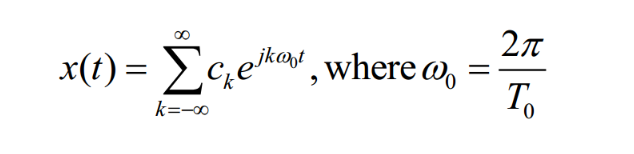
\includegraphics[width=0.3\linewidth]{p6}
	\label{fig:p6}
\end{figure}
The coefficients
$c_k$ in the above equation can be calculated by the analysis
equation,
\begin{figure}[H]
	\centering
	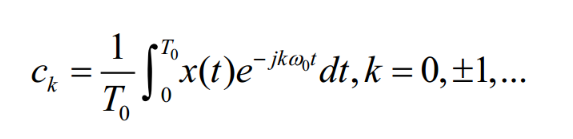
\includegraphics[width=0.3\linewidth]{p7}
	\label{fig:p7}
\end{figure}
\begin{figure}[H]
	\centering
	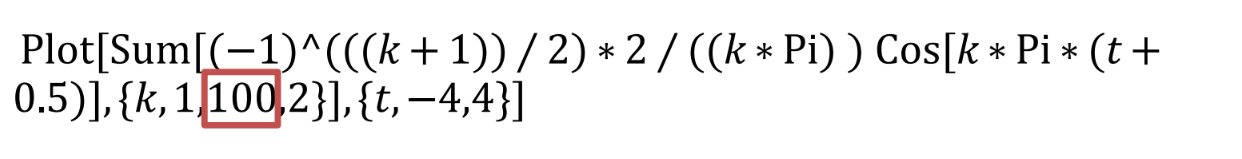
\includegraphics[width=0.4\linewidth]{p8}
	\label{fig:p8}
\end{figure}
\begin{figure}[H]
	\centering
	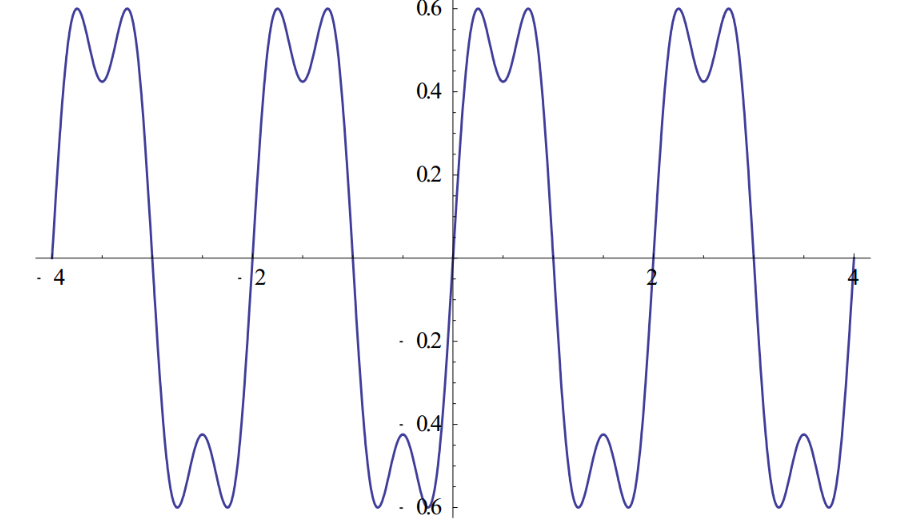
\includegraphics[width=0.7\linewidth]{p9}
	\label{fig:p9}
\end{figure}
For value 20, we can get the following result,
\begin{figure}[H]
	\centering
	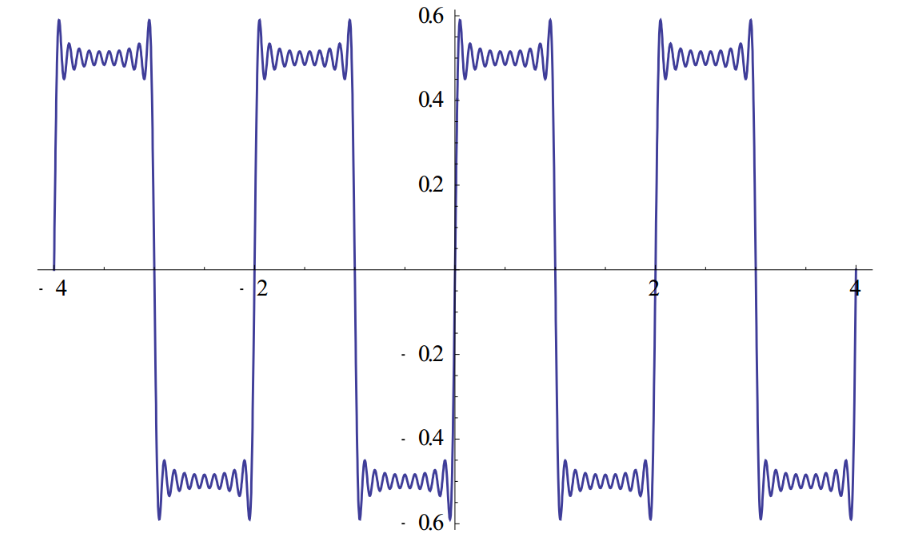
\includegraphics[width=0.7\linewidth]{p10}
	\label{fig:p10}
\end{figure}
And for value 100, we get,
\begin{figure}[H]
	\centering
	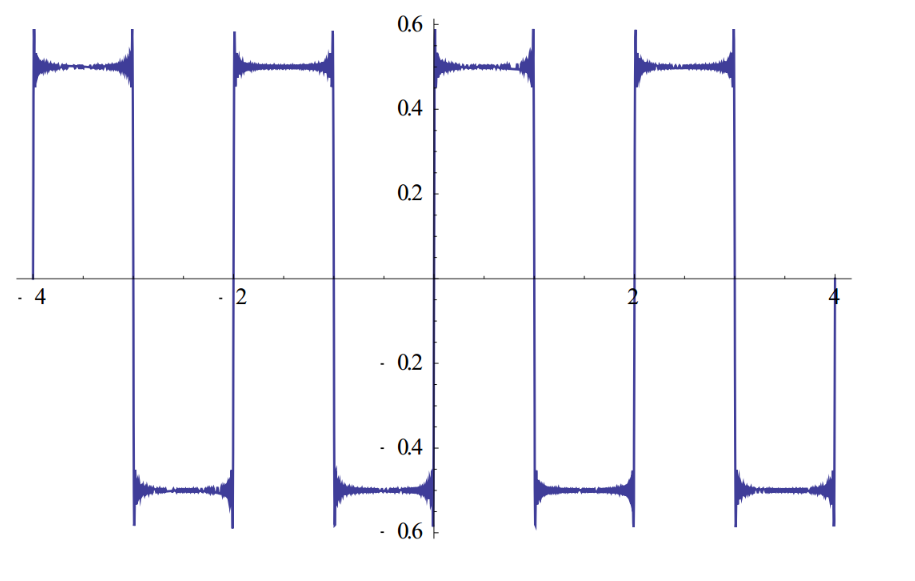
\includegraphics[width=0.7\linewidth]{p11}
	\label{fig:p11}
\end{figure}
\subsubsection{Four ways to measure the amplitude of a sinusoid}
\begin{enumerate}
	\item $V_{peak}=V_{p}=V_{pk}=V_0$ is the peak amplitude of the sinusoid measured in V or mV
	\item $V_{peak-to-peak}=V_{ppk}=V_{max}-V_{min}=2V_0$ is the value we often use in the lab to
	determine the overall size of the waveform. We have used it many times in the previous Labs.
	\item $V_{RMS}$ is the Root-Mean-Square, or RMS amplitude of the sinusoid. The
	sinusoidal voltage $V=V_0sin(\omega t+\theta)$ dissipates as much power in the load resistor
	as does the DC voltage equals to $V_{RMS}$
	\begin{figure}[H]
		\centering
		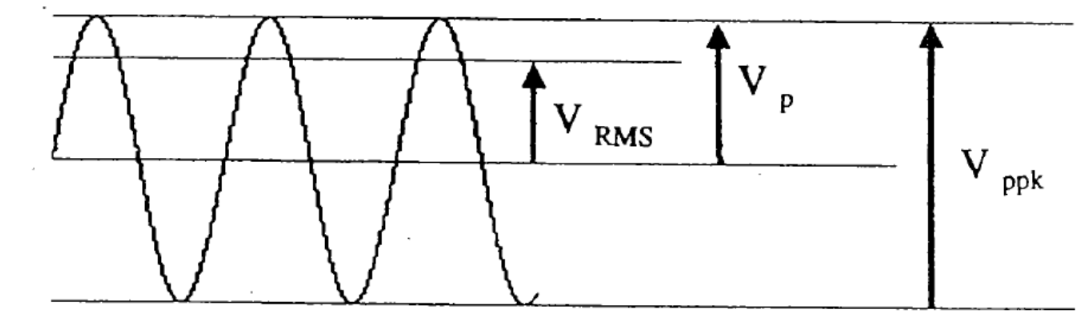
\includegraphics[width=0.7\linewidth]{p12}
		\label{fig:p12}
	\end{figure}
	For any periodic function $f(t)$ that has period T, the RMS amplitude is defined as
	\begin{figure}[H]
		\centering
		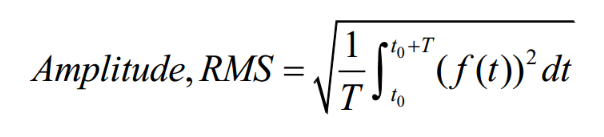
\includegraphics[width=0.4\linewidth]{p13}
		\label{fig:p13}
	\end{figure}
In the case of sinusoid $f(t)=V_0sin(\omega t+\theta)$
\begin{figure}[H]
	\centering
	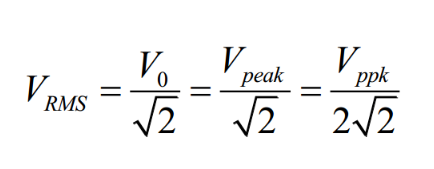
\includegraphics[width=0.3\linewidth]{p14}
	\label{fig:p14}
\end{figure}
\item The above three ways all study the signal in time domain, plotted as voltage vs.
time. In this Lab, we also need to study the frequency domain, when you measure
their spectra displayed as amplitude vs. frequency. In frequency domain, the
oscilloscope measures the amplitude of on a logarithmic scale, using decibels.
\begin{figure}[H]
	\centering
	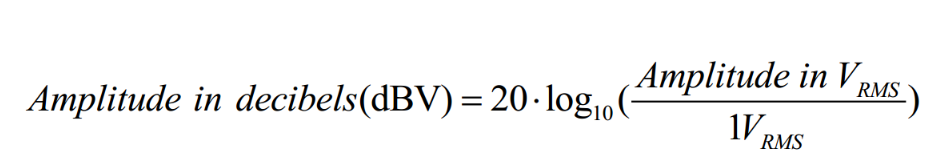
\includegraphics[width=0.6\linewidth]{p15}
	\label{fig:p15}
\end{figure}
Decibels are used to calculate ratios of two amplitudes on a logarithmic scale.
\begin{figure}[H]
	\centering
	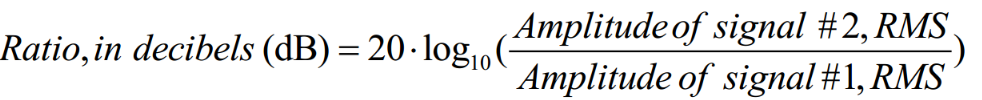
\includegraphics[width=0.7\linewidth]{p16}
	\label{fig:p16}
\end{figure}
\end{enumerate}
\section{Procedure}
\subsection{Part 1}
\begin{enumerate}
	\item On the function generator, set a sine wave at 1 [kHz] and keep its amplitude
	at 3 [Vpp]. The load must be High-Z mode.
	\item Record the parameters on the datasheet. Fill the table with the data set on the
	function generator and displayed on the oscilloscope.
	\item Repeat the Step 2 with a sine wave at 1.5 [kHz] and 5 [Vpp] on the function
	generator. The load should remain High-Z mode.
	\item In post-report, calculate the rise time in theory and compare it with the values
	displayed on the oscilloscope.
	\item Reminder: $RiseTime=\frac{[sin^{-1}(\frac{V_{min}+0.9V_{pp}}{0.5V_{PP}})-sin^{-1}(\frac{V_{min}+0.1V_{pp}}{0.5V_{PP}})]}{2\pi f}$
\end{enumerate}
\subsection{Part 2}
\begin{enumerate}
	\item First, we set a sine wave and a square wave, respectively. The frequency is 1
	[kHz] and the amplitude is 3 [Vpp].
	\item On the oscilloscope, set 1 [V/div] and 5 [ms/div].
	\item Push the “MATH” button and select “FFT” function.
	\item Push the “cursor” button and select “trace” mode to trace the spectrum.
	\item When the cursor reach a peak of the spectrum, record the Frequency in [kHz]
	and the Amplitude in [dBV].
	\item Set another sine wave and a square wave. The frequency is 2 [kHz] and the
	amplitude is 6 [Vpp]. Repeat the steps above.
	\item In post-report, you need to calculate the theoretical amplitude of sine wave in
	[dBV]. Besides, you need to calculate the Vpeak of each square wave
	measured in Part II. You should give a brief conclusion on what you learn
	from this lab.
	\item Reminder: for sine wave $dBV=20log(\frac{AmplitudeinV_{RMS}}{1V_{RMS}})$
	\item Reminder: for square wave $V_{peak}=\sqrt{2}\cdot 10(\frac{Amplitude in [dBV]}{20})$
\end{enumerate}
\section{Part 1}
\begin{table}[H]
	\centering
\begin{tabular}{|c|c|c|}
	\hline 
	& Set on Function Generator & Measured with Oscilloscope \\ 
	\hline 
	Amplitude& 3 & 3.1 \\ 
	\hline 
	Frequency [kHz]& 1 & 1 \\ 
	\hline 
	Rise Time [$\mu s$]&  & 280 \\ 
	\hline 
	Amplitude in Vpp [V]& 5 & 5.15 \\ 
	\hline 
	Frequency [kHz]& 1.5 & 1.5 \\ 
	\hline 
	Rise Time [$\mu s$]&  & 190 \\ 
	\hline 
\end{tabular} 
\caption{Rise Time Measurement}
\end{table}
The theoretical time of the Amplitude 3 Frequency 1 is 295. It seems that the error is not very big. The absolute error is $295-280=15$. Then the relative error is $\frac{295-280}{280}\times 100\%=5.4\%$

The theoretical time of the Amplitude 5 Frequency 1.5 is 197. It seems that the error is not very big. The absolute error is $197-190=7$. Then the relative error is $\frac{197-190}{197}\times 100\%=3.6\$$
\section{part 2}
\subsection{3 [Vpp] 1 [kHz]}
\begin{table}[H]
	\centering
	\begin{tabular}{|c|c|c|}
		\hline 
		Peak& Frequency (measured) [kHz] & Amplitude (measured) [dBV] \\ 
		\hline 
		$f_0$&1  & -0.150 \\ 
		\hline 
	\end{tabular} 
\caption{FFT spectrum for Sine wave}
\end{table}
The theoretical value of the amplitude of the sine wave is about 0.51. $20log(\frac{3}{2\sqrt{2}})=0.51$ And we find that the error is a little bit large. I think the reason is that the theoretical value is not very big. The absolute error is 0.660. The relative error is $\frac{0.51-(-0.15)}{0.51}\times 100\%=129\%$. It seems that the error of this experiment is big.
\begin{table}[H]
	\centering
	\begin{tabular}{|c|c|c|}
		\hline 
		Peak& Frequency (measured) [kHz] & Amplitude (measured) [dBV] \\ 
		\hline 
		$f_0$& 1 & 1.74 \\ 
		\hline 
		$3f_0$& 3 & -7.704 \\ 
		\hline 
		$5f_0$& 5 & -12.110 \\ 
		\hline 
		$7f_0$& 7 & -14.989 \\ 
		\hline 
		$9f_0$& 9 & -17.145 \\ 
		\hline 
	\end{tabular} 
\caption{FFT spectrum for Square Wave}
\end{table}
\begin{table}[H]
	\centering
	\begin{tabular}{|c|c|c|c|}
		\hline 
		Peak& Frequency (measured) [kHz] & Amplitude (measured) [dBV] &Amplitude (theoretical) [dBV]\\ 
		\hline 
		$f_0$& 1 & 1.74 &2.610\\ 
		\hline 
		$3f_0$& 3 & -7.704&-6.933 \\ 
		\hline 
		$5f_0$& 5 & -12.110&-11.370 \\ 
		\hline 
		$7f_0$& 7 & -14.989&-14.292\\ 
		\hline 
		$9f_0$& 9 & -17.145 &-16.475\\ 
		\hline 
	\end{tabular} 
	\caption{FFT spectrum for Square Wave (2)}
\end{table}
\begin{table}[H]
	\centering
	\begin{tabular}{|c|c|c|c|}
		\hline 
		Peak& Frequency (measured) [kHz] & Amplitude (measured) [dBV] &$V_{peak}$\\ 
		\hline 
		$f_0$& 1 & 1.74 &1.73\\ 
		\hline 
		$3f_0$& 3 & -7.704&0.58 \\ 
		\hline 
		$5f_0$& 5 & -12.110&0.35 \\ 
		\hline 
		$7f_0$& 7 & -14.989&0.25\\
		\hline 
		$9f_0$& 9 & -17.145 &0.20\\ 
		\hline 
	\end{tabular} 
	\caption{FFT spectrum for Square Wave (2)}
\end{table}
\subsection{6 [Vpp] 2 [kHz]}
	\begin{table}[H]
		\centering
		\begin{tabular}{|c|c|c|}
			\hline 
			Peak& Frequency (measured) [kHz] & Amplitude (measured) [dBV] \\ 
			\hline 
			$f_0$&2  & 5.817 \\ 
			\hline 
		\end{tabular} 
		\caption{FFT spectrum for Sine wave}
	\end{table}
The theoretical value of this experiment is 6.53. $20log(\frac{6}{2\sqrt{2}})=6.53$ Our result is very close to the theoretical value. The absolute error is 0.713. The relative error is about $\frac{(6.53-5.817)}{6.53}\times 100\%=10.9\%$. This result is much better then the previous one.
	\begin{table}[H]
		\centering
		\begin{tabular}{|c|c|c|}
			\hline 
			Peak& Frequency (measured) [kHz] & Amplitude (measured) [dBV] \\ 
			\hline 
			$f_0$& 2 & 7.926 \\ 
			\hline 
			$3f_0$& 6 & -1.630 \\ 
			\hline 
			$5f_0$& 10 & -6.061 \\ 
			\hline 
			$7f_0$& 14 & -9.010 \\ 
			\hline 
			$9f_0$& 18 & -11.141 \\ 
			\hline 
		\end{tabular} 
		\caption{FFT spectrum for Square Wave}
	\end{table}
	\begin{table}[H]
		\centering
	\begin{tabular}{|c|c|c|c|}
		\hline 
		Peak& Frequency (measured) [kHz] & Amplitude (measured) [dBV] &Amplitude (theoretical) [dBV]\\ 
		\hline 
		$f_0$& 2 & 7.926 &8.30\\ 
		\hline 
		$3f_0$& 6 & -1.630 &-0.912\\ 
		\hline 
		$5f_0$& 10 & -6.061 &-5.439\\ 
		\hline 
		$7f_0$& 14 & -9.010 &-8.272\\ 
		\hline 
		$9f_0$& 18 & -11.141 &-10.455\\ 
		\hline 
	\end{tabular} 
	\caption{FFT spectrum for Square Wave (2)}
\end{table}
\begin{table}[H]
	\centering
	\begin{tabular}{|c|c|c|c|}
		\hline 
		Peak& Frequency (measured) [kHz] & Amplitude (measured) [dBV] &$V_{peak}$\\ 
		\hline 
		$f_0$& 2 & 7.926 &3.522\\ 
		\hline 
		$3f_0$& 6 & -1.630 &1.172\\ 
		\hline 
		$5f_0$& 10 & -6.061 &0.704\\ 
		\hline 
		$7f_0$& 14 & -9.010 &0.50\\ 
		\hline 
		$9f_0$& 18 & -11.141 &0.39\\ 
		\hline 
	\end{tabular} 
	\caption{FFT spectrum for Square Wave (2)}
\end{table}
\section{conclusion}


We learn  how to define, calculate, and measure the amplitude of a sinusoidal
signal,  how to define, calculate, and measure the Rise Time and Fall Time of a
signal, how to observe FFT spectra of signal and measure their parameters with
cursors, measure the waveforms and FFT spectra of various signals and compare your theoretical results obtained in the Pre-Lab with your In-Lab
data.

In the first part, we measured the characteristics of a sine AC source. And in the second part, we learned the FFT spectrum for Square Wave.

From this experiment, we find that it is relatively easy to get a relative correct result. And from the data of our experiment, we find that it is relatively correct, and there aren't many very big mistakes. 
\end{document}